\section{Perceived quality measurement}

In this section we first introduce Peak Signal-to-Perceptible-Noise Ratio (PSPNR) \cite{PSPNR} which is used as metric for perceived quality measurement. Then, since PSPNR computation needs the Just-Noticeable-Distortion (JND) \cite{JND} value of each pixel, we present our JND definition based on human visual system in VR display.

\subsection{Perceived quality measuring by Just-Noticeable Distortion (JND) model}

Since user-perceived quality is a subjective thing, how to measure it becomes a problem. For example, it is very hard for a user to say the perceived quality of video A is 2 times better than that of video B, or it is just 1.7 times better.

Peak Signal-to-Perceptible-Noise Ratio (PSPNR) \cite{PSPNR} is an widely-accepted metric to measure perceived quality. It is defined based on Just-Noticeable-Distortion (JND) theory \cite{JND}. Given the original video frame and a compressed video frame, user can notice their difference only if the difference between them is above a visibility threshold. When the different is under this threshold, it will not detected by user. This threshold is called Just-Noticeable-Distortion.

Based on JND theory, PSPNR is defined by accumulating error of each pixel which can be detected by user:

\begin{alignat}{2}\
\label{f1} PSPNR = 20 \times \log_{10}\frac{255}{\sqrt{PMSE}}
\end{alignat}
\begin{alignat}{2}\
PMSE=E\{ \left[ |p(x, y) - \hat{p}(x, y)| - JND(x, y)\right]^2 \times \Delta (x, y)\}
\end{alignat}
\begin{alignat}{2}\
\Delta (x, y) =\left\{
\begin{aligned}
1, & &|p(x, y) - \hat{p}(x, y)| > JND(x, y) \\
0, & &|p(x, y) - \hat{p}(x, y)| \le JND(x, y)
\end{aligned}
\right.
\end{alignat}

where $p(x, y)$ and $\hat{p}(x, y)$ are value of pixel $(x, y)$ in original video frame and compressed video frame. $JND(x, y)$ is the visibility threshold of pixel $(x, y)$.

Compared with PSNR (which is widely used in evaluating video / image quality), the core difference of PSPNR is introducing a term $JND(x, y)$ for each pixel $(x, y)$. So how to compute JND for each pixel $(x, y)$ is an important issue. We will present our JND computation in the following section.

\subsection{Building Just-Noticeable-Distortion Model for VR display}
The just-noticeable distortion (JND) provides cues for measuring the visibility of the Human Vision System (HVS). JND refers to the maximum distortion which cannot be perceived by human. It describes the perceptual redundancy of the picture by providing the visibility threshold. The JND model generally exploits the visibility of the minimally perceptible distortion.

JND has been well-studied in traditional video display since 1995. The most basic and solid research is about the relationship between content luminance and JND. \cite{luminance1}  and \cite{PSPNR} prove that content with moderate content luminance have low JND value, while content with very high or very low content luminance have high JND value. (Fig. \ref{JNDluminance})

\begin{figure}
  \centering
  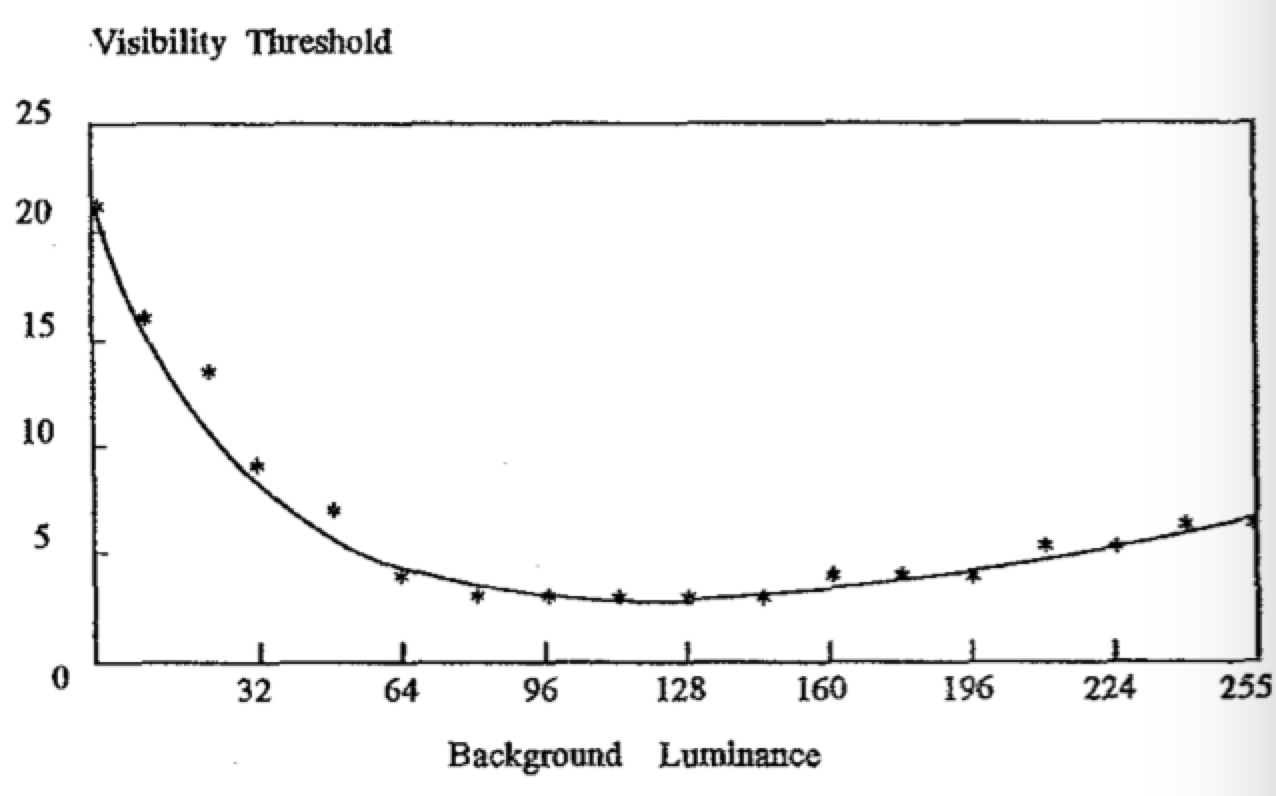
\includegraphics[width=2.5in]{images/backgroundluminance.jpg}
  \caption{JND due to content luminance.}
  \label{JNDluminance}
  \end{figure}

In recent years, based on the insight of content luminance - JND relationship, researchers have explored some more factors which are also related to JND, such as texture complexity, viewpoint-object distance (\cite{PSPNR}, \cite{distance}) and some other factors. Although the relationship between multiple JND factors may be complex, for simplicity, we can decouple them into several single factors. For example, \cite{distance} set up a user study to test the JND value with the combined effect of content luminance and viewpoint-object distance. The result proves that viewpoint-object distance can be considered independently from content luminance (Fig. \ref{JNDlum-dist}). It can be regarded as a coefficient which can be directly multiplied on JND value computed by content luminance. Based on this insight, JND computation for multiple factors is decoupled into several single factors. This significantly simplify the JND computation.

\begin{figure}
  \centering
  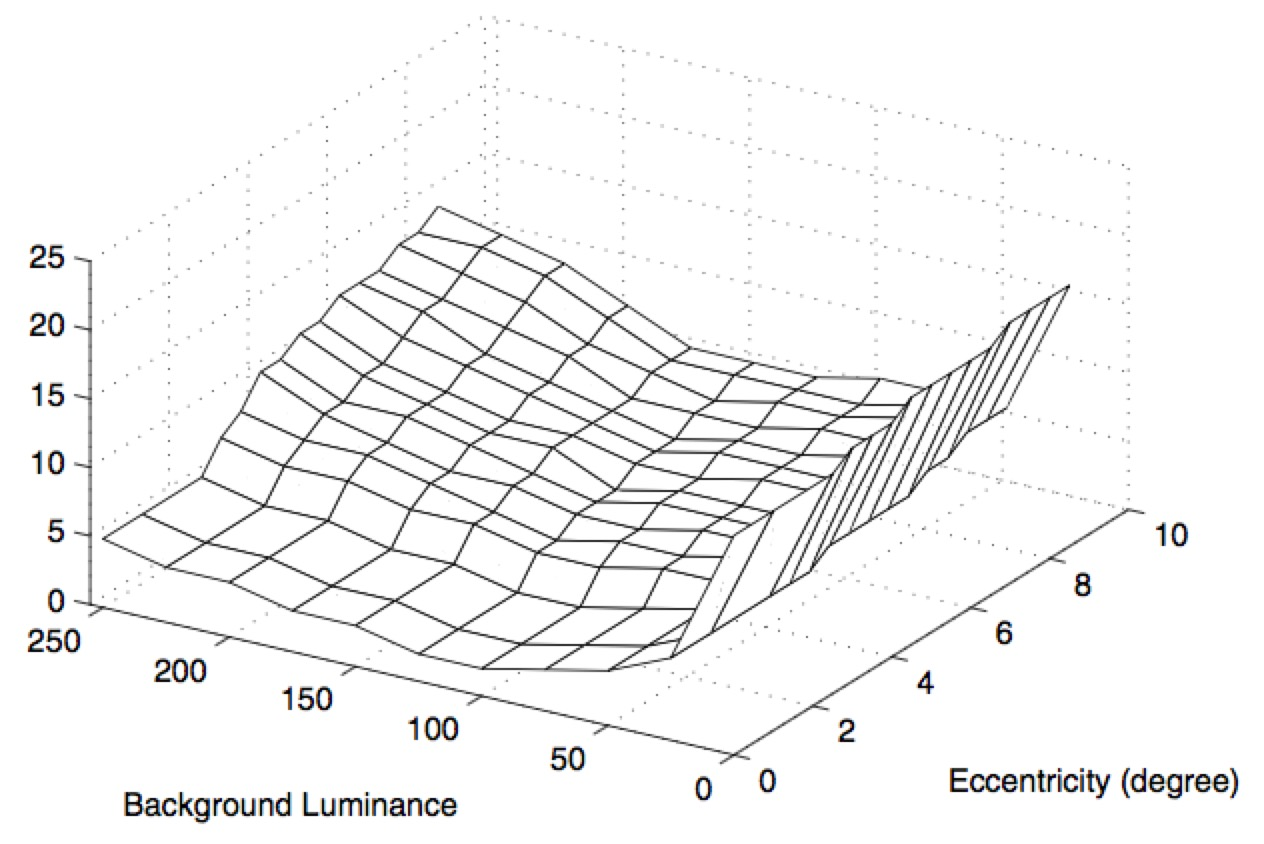
\includegraphics[width=2.5in]{images/JNDlum-dist.jpg}
  \caption{JND due to content luminance \& viewpoint-object distance.}
  \label{JNDlum-dist}
  \end{figure}

In VR display, user experience is very different because 3 new factors should be taken into consideration: (1) viewpoint moving decreases visual acuity, (2) low Depth-of-Field decreases visual acuity and (3) light / dark adaptation decreases visual acuity. So previous JND model for traditional video display can not be directly applied on VR video display. Moreover, it is unknown that (1) how these new factors influence JND with combined effect of old factors, and (2) if they can also be decoupled into several single factors, like viewpoint-object distance \cite{distance}.

Strictly answering these 2 questions needs to test JND value for each possible combinations of all factors (including all possible luminance, texture, viewpoint-object distance, viewpoint moving speed, Depth-of-Field and light / dark adaptation, which make up a 6-dimension feature space), which is not practical for a real-world user study. For simplicity, we imitate the user study in \cite{distance}, which makes only 2 factors variable and other 4 factors fixed, then we can know how is the combined effect of the 2 factors to JND, and if they can be decoupled to 2 single factors which independently influence JND.

So we present 3 user studies: (1) JND v.s. luminance \& viewpoint moving speed. (2) JND v.s. luminance \& depth of field. (3) JND v.s. luminance \& light / dark adaptation. We evaluate the effect of 3 VR-only factors to JND, each with combined effect of luminance, since luminance is the most well-studied JND factor.

We conduct the user study using real Head Mounted Device (HMD). Parameters of proposed HMD are listed as Table \ref{table1}:

\begin{table}[h]
\centering
\caption{HMD Parameters}\label{table1}
\begin{tabular}{|p{3.5cm}|p{3.5cm}|}
\hline
Equipment & Oculus GO\\
CPU & Xiaolong 821 customized drive Edition\\
Memory & 3GB\\
Screen Resolution & 2560 $\times$ 1440\\
Refresh Rate & 72Hz\\
Fixed pupil distance & 63.5mm\\
\hline
\end{tabular}
\end{table}

20 subjects participated in the experiments. All of them were in their twenties. The subjects obtained extensive practice during the experiments.

In this paper, we imitate the human visibility experiments in \cite{PSPNR}. In the experiment, a small square area, 32 x 32 pixels, is located in the center of a flat field of constant grey level (luminance). For each possible grey level (luminance) of the square area, the noises of fixed amplitude are randomly added to or subtracted from the pixels within the square area. Through varying the amplitude of the noise, the visibility threshold for each grey level is determined when the square region contaminated by the noises is just noticeable. 

Experimental settings of our 3 user studies are:

1. \textbf{JND v.s. luminance \& viewpoint moving speed} Set a background with constant grey level and set the 32 * 32 square with 5 different grey levels: 30, 80, 130, 180 and 230. The square is doing uniform rectilinear motion on the background. Noises are randomly added to or subtracted from it. We test the visibility threshold in 2 conditions: (1) Observer's viewpoint is gazed on a fixed point and the square moves across the fixed point. (set the moving speed of 32*32 square area to 2 deg /s, 4 deg / s, 6 deg / s, 8 deg / s, 10 deg / s) (2) Observer's viewpoint is allowed to tracking the moving object. (set the moving speed of 32*32 square area to 5 deg /s, 10 deg / s, 20 deg / s, 40 deg / s, 80 deg / s)

2. \textbf{JND v.s. luminance \& depth of field} Set a background with constant grey level and set the 32 * 32 square with 5 different grey levels: 30, 80, 130, 180 and 230. Then set the depth-of-field of the square to 1m, 1.5m, 3m, 50m. Testing the visibility threshold for these situations.

3. \textbf{JND v.s. luminance \& light / dark adaptation} Before our test, we show subjects a pure background with gray level $L_A$ ($L_A$ = 30, 80, 130, 180, 230) for 20 seconds. Then we change the background gray level to $L_B$ ($L_B$ = 30, 80, 130, 180, 230) and show subjects the 32*32 square. Testing the visibility threshold for these situations.

As described above, our user study contains multiple independent repetitive experiments. But we have stated that perceived quality is related to human visual system and human brain (\S 2), and human brain can be trained during the experiment. So long-time continuous experiment may make subjective more and more skillful, which leads to elimination of JND difference in different situation, and decreasing value of JND during the process of experiment. To eliminate the impair of this, we (1) dispart the experiment into 3 days, with only 5 minutes for each day. (2) random the test order of each single test.

\subsection{Results}

\subsubsection{JND v.s. luminance \& viewpoint moving speed}

One of the most highlighted feature of VR video is that users can freely move their viewpoints. According to our data analysis, more than 30\% viewpoints are moving faster than 20 deg/s. (Fig. \ref{CDFspeed}) When human viewpoint is moving, visual acuity is decreased in 2 different conditions: (1) if user is tracking an object, visual acuity decreases smoothly with viewpoint moving speed increases. (2) If user is not tracking an object, visual acuity decreases dramatically with viewpoint moving speed increases. \cite{speed}

\begin{figure}
  \centering
  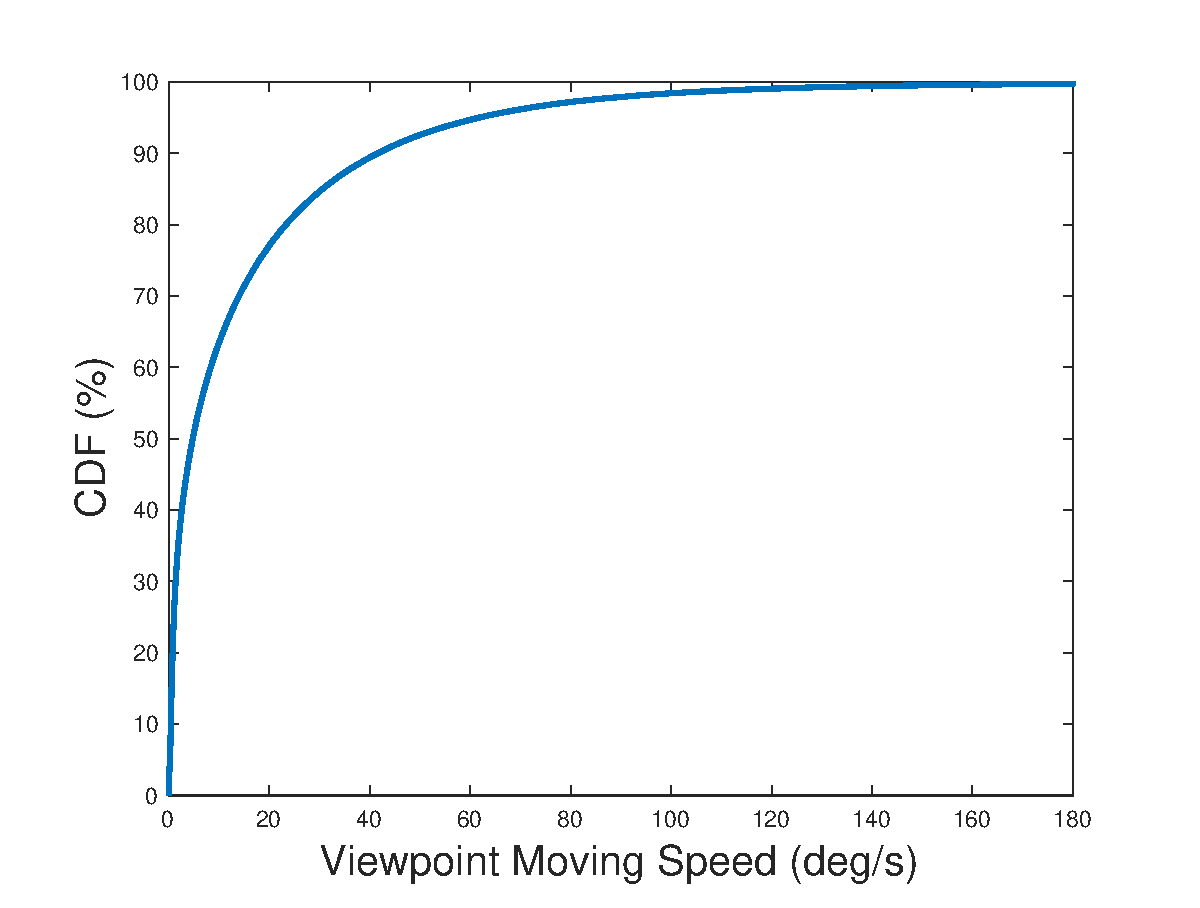
\includegraphics[width=2.5in]{images/speed_CDF.eps}
  \caption{CDF gram of viewpoint moving speed.}
  \label{CDFspeed}
  \end{figure}
  
We first analyze tracking condition. Fig. \ref{JNDspeed-lum-track} shows $JND_{lum\&speed}^{track}(l, v)$, the combined effect of viewpoint moving speed $v$ and content luminance $l$ to JND. We notice that effect of $v$ to $JND_{lum\&speed}^{track}$ is very similar in different $l$, so this combined effect can be decoupled into 2 parts:

\begin{figure}
  \centering
  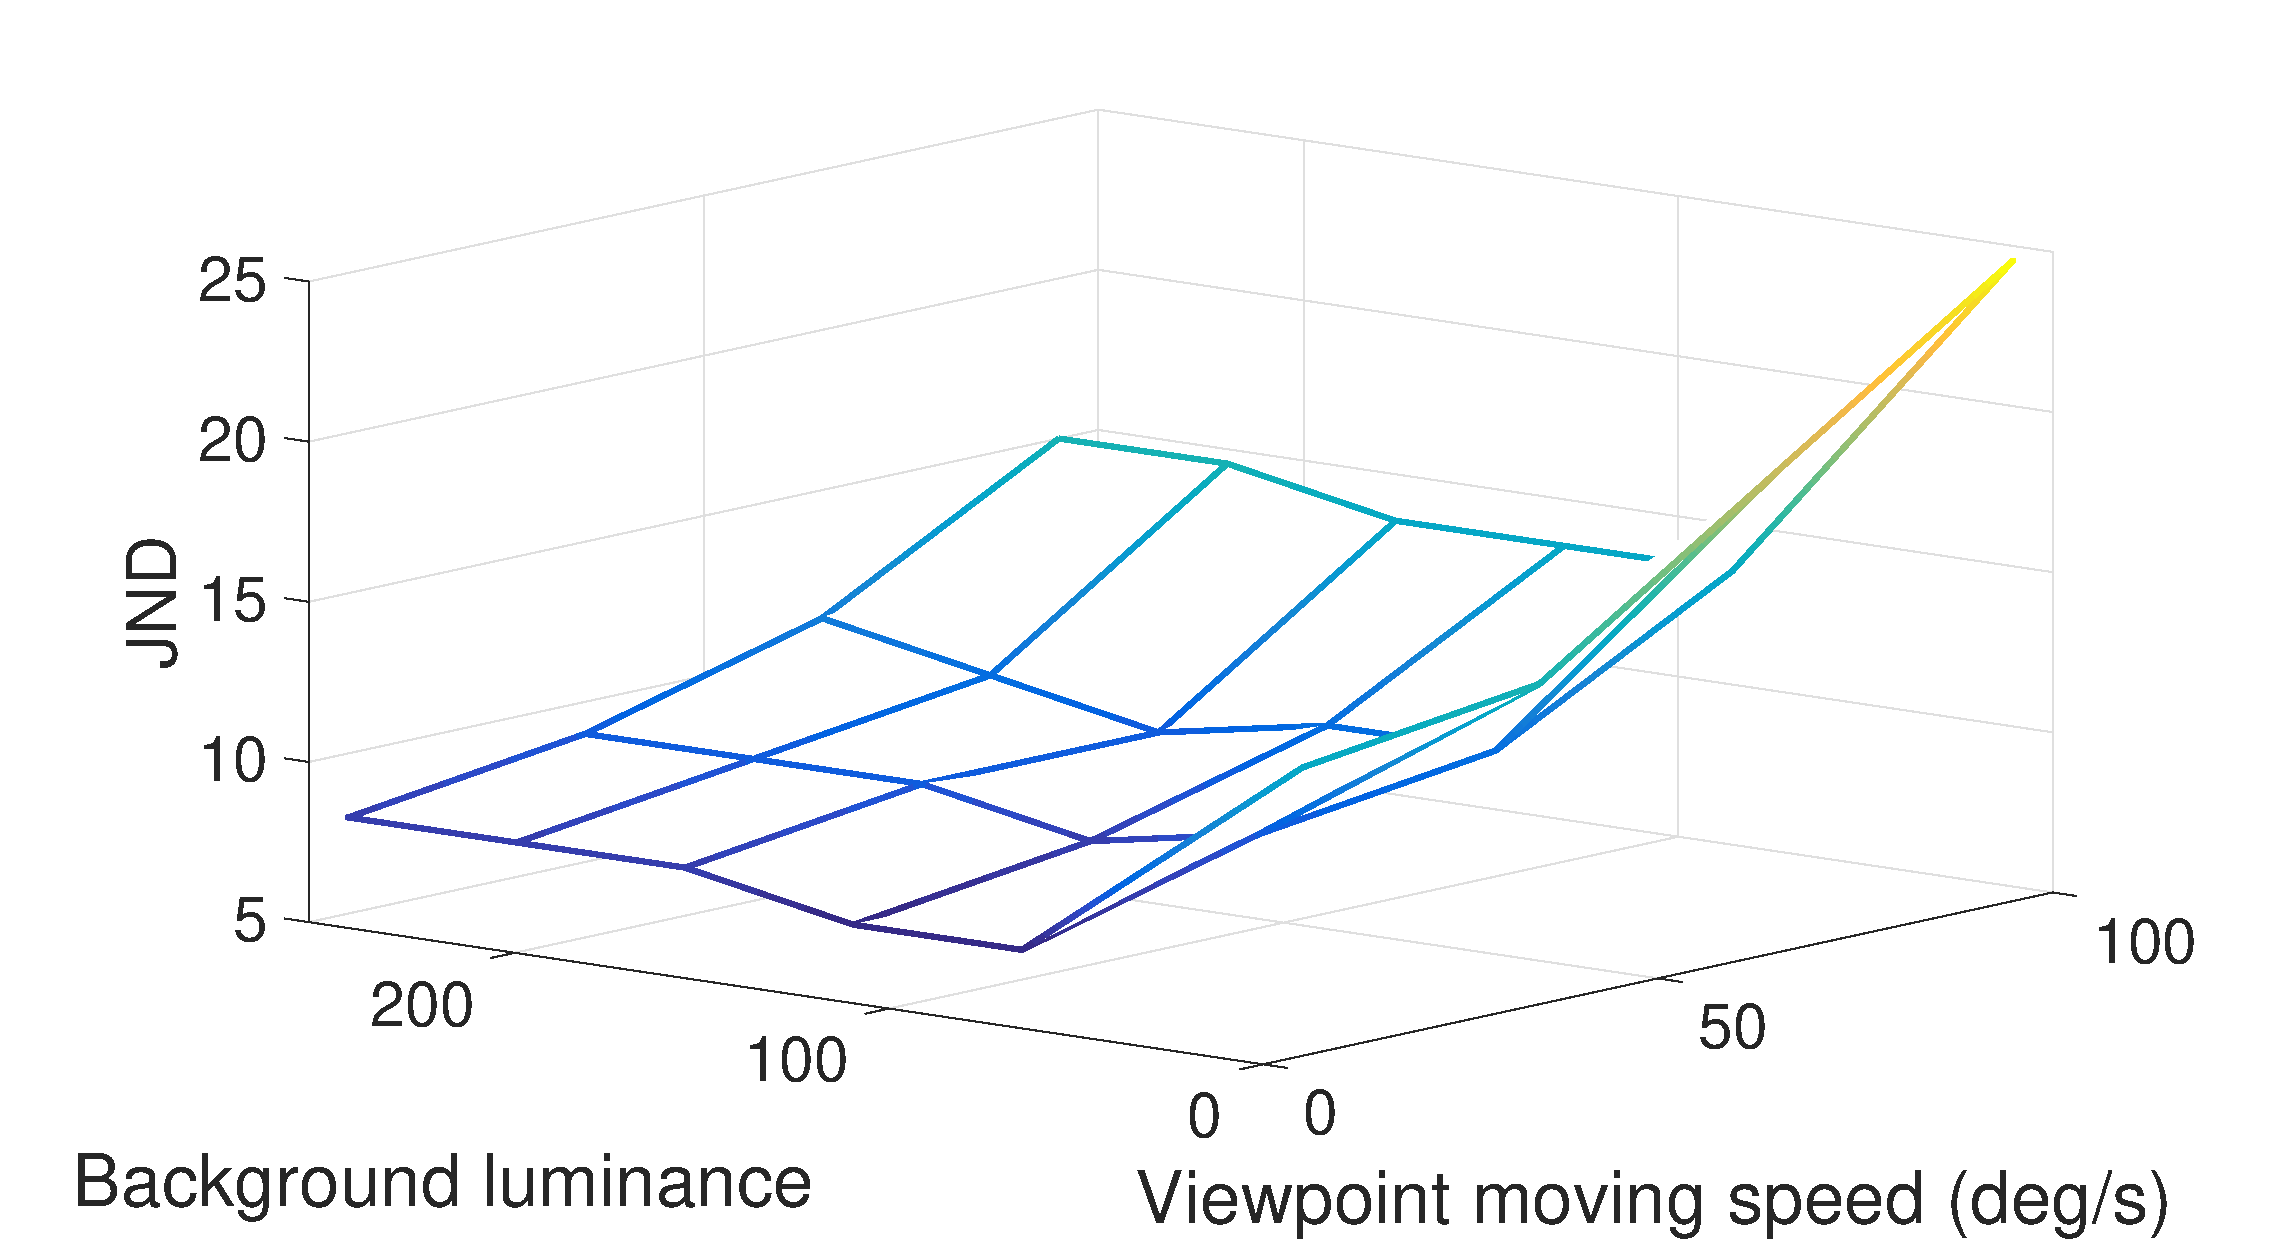
\includegraphics[width=2.5in]{images/JNDspeed-lum.eps}
  \caption{JND due to content luminance and viewpoint moving speed.}
  \label{JNDspeed-lum-track}
  \end{figure}

\begin{alignat}{2}\
JND_{lum\&speed}^{track}(l, v) = f_{lum}(l) \times f_{track}(v)
\end{alignat}

where $f_{lum}(l)$ represents the visibility threshold with only consideration of content luminance, and $f_{track}(v)$ is a coefficient which represents influence of viewpoint moving speed on visibility threshold.

$f_{lum}(l)$ has been presented as Fig. \ref{JNDluminance}. According to curve fitting, we can obtain $f_{track}(v) = \frac{JND_{lum\&speed}^{track}(l, v)}{f_{lum}(l)}$ as Fig. \ref{JNDspeed-track}.

\begin{figure}
  \centering
  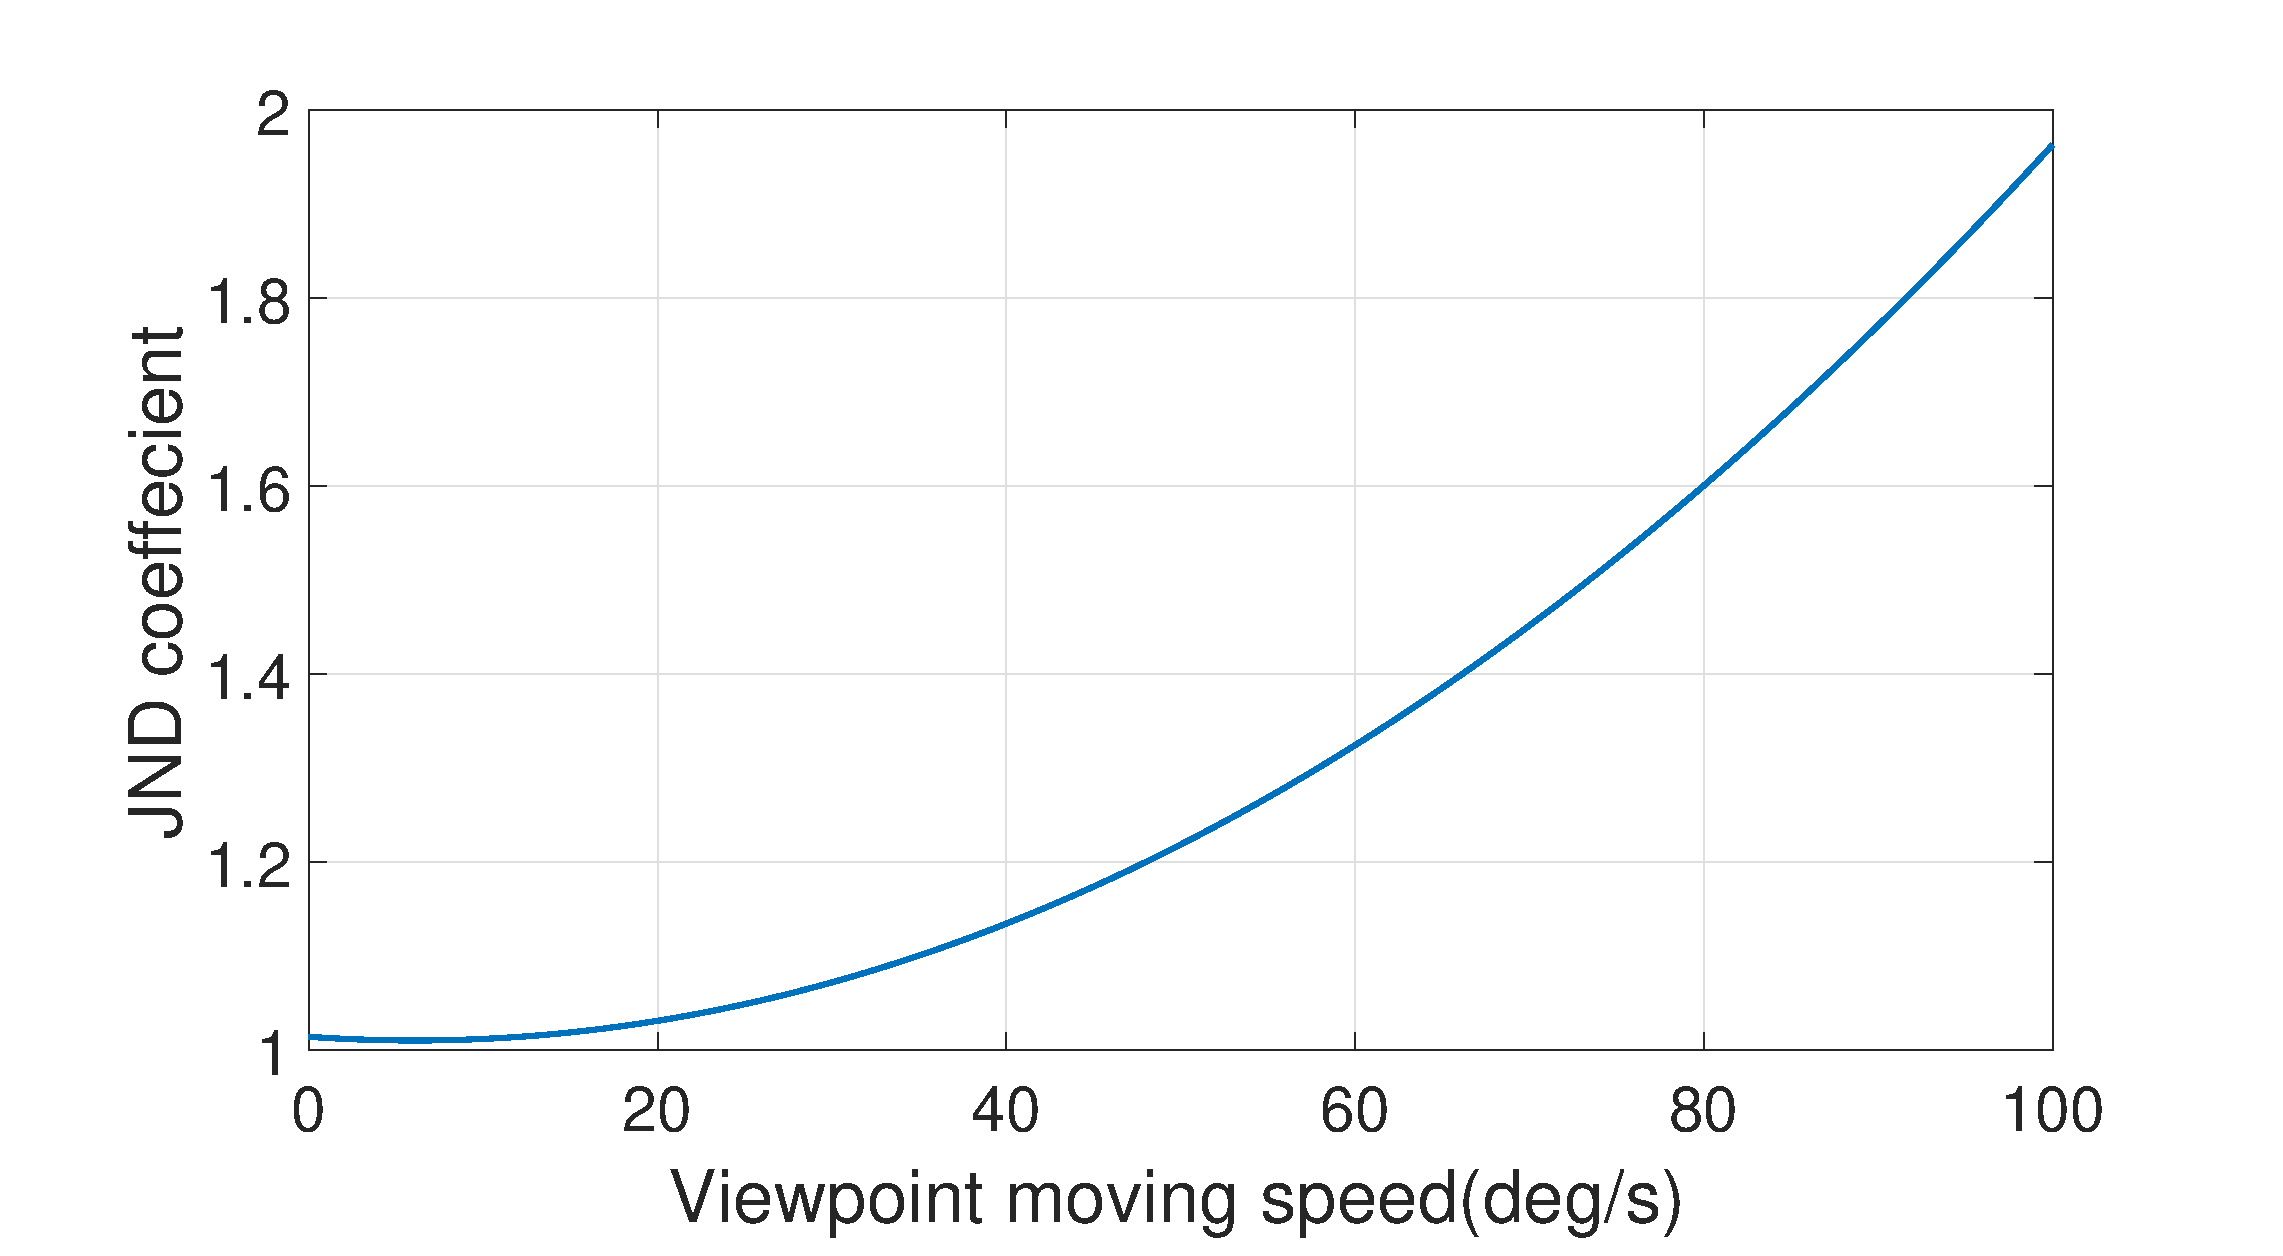
\includegraphics[width=2.5in]{images/JNDspeed.eps}
  \caption{$f_{track}(v)$, the JND coefficient of viewpoint moving speed.}
  \label{JNDspeed-track}
  \end{figure}

With similar method, we obtain result of no-tracking condition, $f_{notrack}(v)$, as Fig. \ref{JNDspeed-notrack}.

\begin{figure}
  \centering
  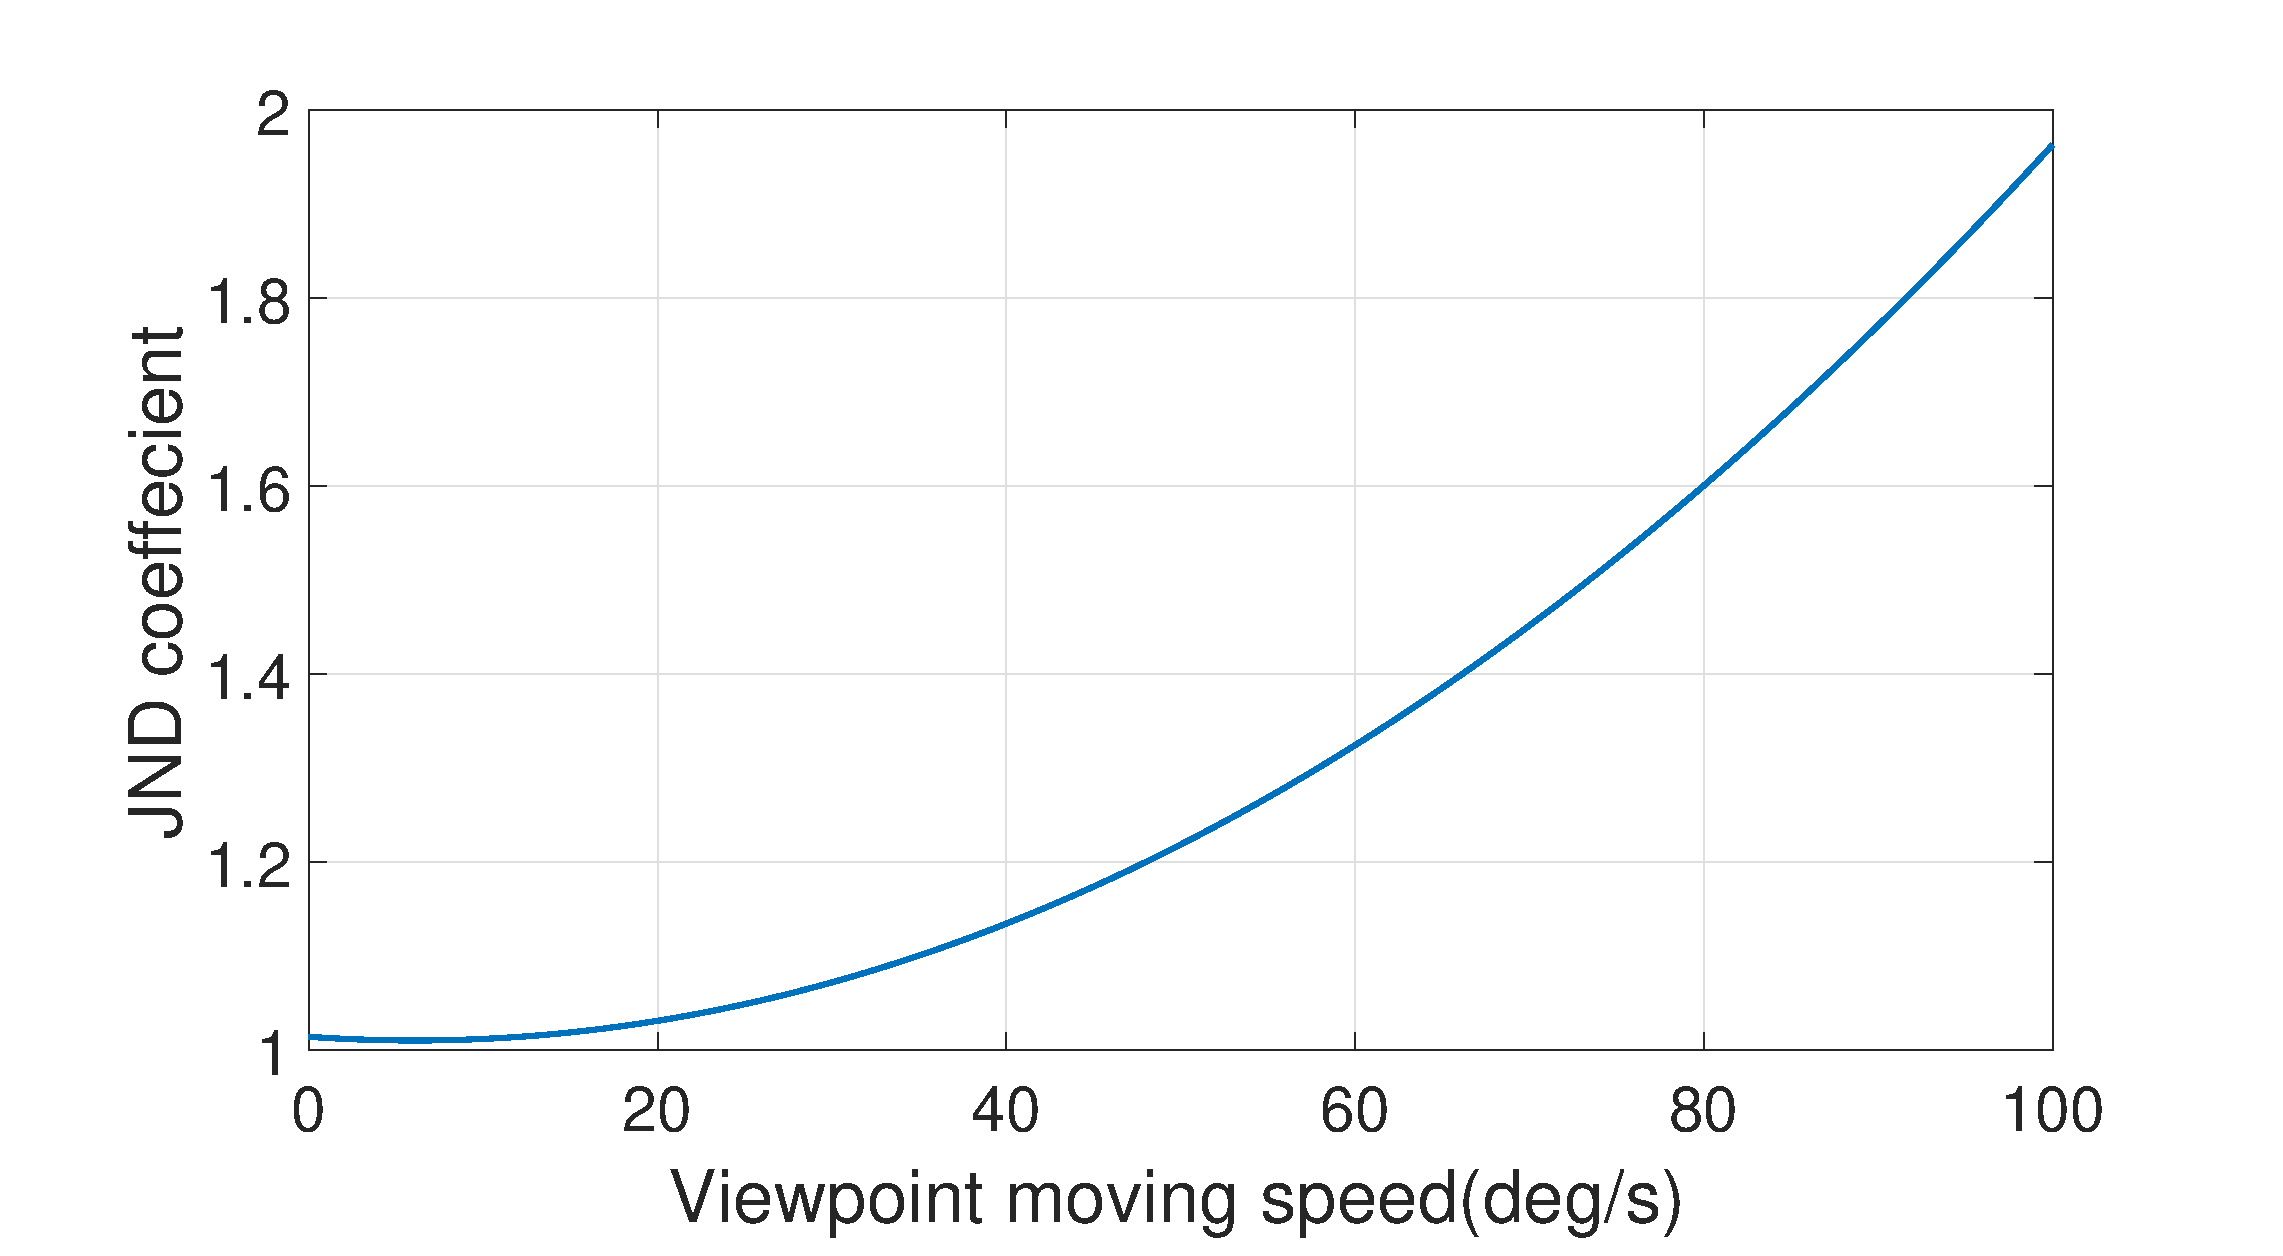
\includegraphics[width=2.5in]{images/JNDspeed.eps}
  \caption{$f_{notrack}(v)$, the JND coefficient of viewpoint moving speed.}
  \label{JNDspeed-notrack}
  \end{figure}

In the real-world, viewpoint moving speed is not given, it needs to be predicted by client-side. Since human action has great randomness, viewpoint moving speed may fluctuate dramatically. It is very difficult to accurately predict user's viewpoint moving speed even in the near future (1s - 5s). Fortunately, since viewpoint moving speed has strong temporal locality, we can easily predict a lower bound of viewpoint moving speed in the near future. Fig. X shows an example of real-world viewpoint moving speed and our predicted viewpoint moving speed by a very simple method. In most of the time, predicted speed does not exceed real speed. So we will not locate the video quality lower than it should be. \S 8 proves that this speed prediction is already enough to cover most of the gain.

\begin{figure}
  \centering
  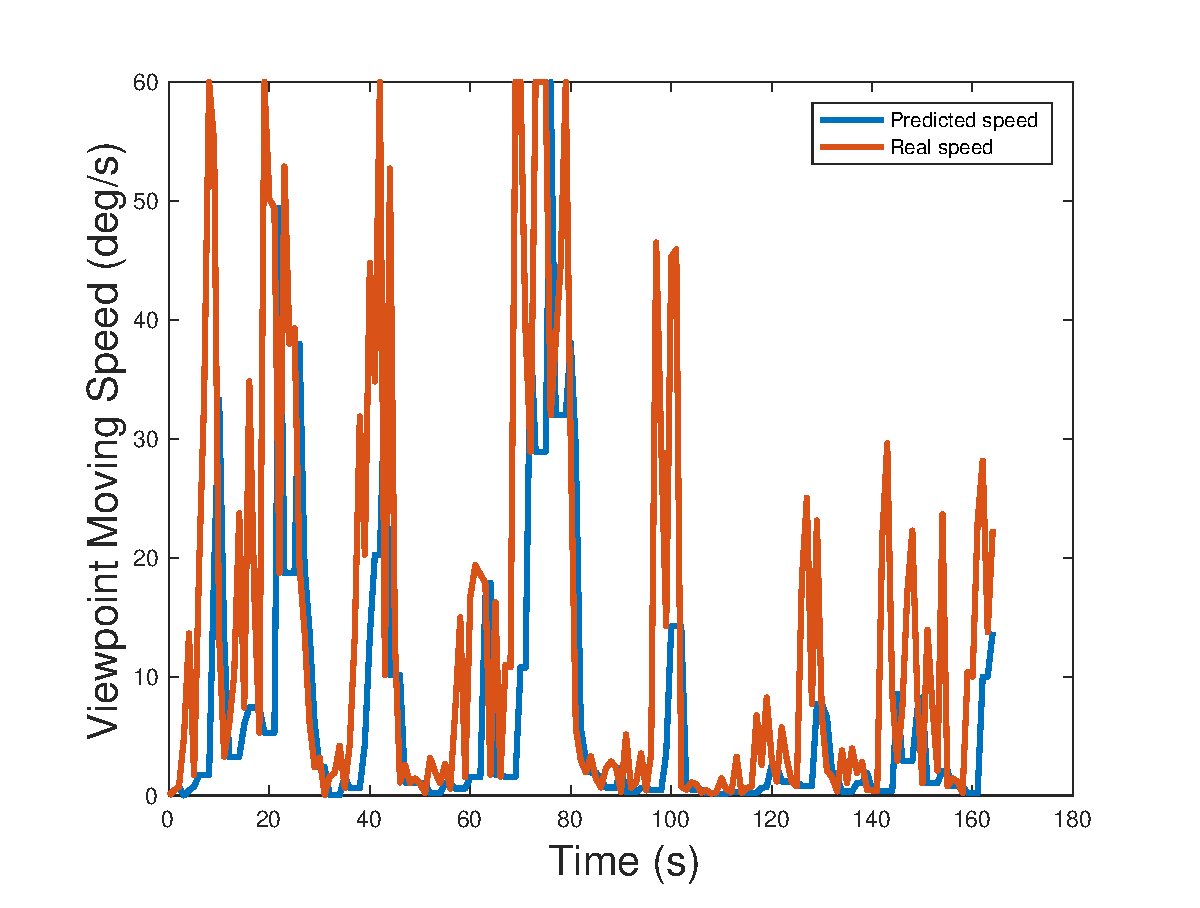
\includegraphics[width=2.5in, height=1in]{images/speed_analysis.eps}
  \caption{An example of real viewpoint moving pattern and predicted viewpoint moving pattern.}
  \label{v-aconflict}
  \end{figure}

\subsubsection{JND v.s. luminance \& depth of field}

Depth-of-field (DoF) refers to the 3D distance from the object to human eyes. In real world, human detect object's DoF by parallax effect (Fig. \ref{v-aconflict}). When a human is focusing on an object, the object's location is different in his left eye and right eye. Then human brain combines 2 different 2D images from 2 eyes and build a 3D image with Depth-of-Field. Plenty of works [] state that DoF influences visual acuity in 2 aspects: (1) Human visibility is weak when focusing on object with small DoF, since combining 2 highly different image from left / right eye is hard and slow. (2) Human visual acuity is weak when focus distance is different from the object's DoF (eg. there are object A and B in a same place but with different DoF, when human is focusing on A, his visual acuity for B is weak).

\begin{figure}
  \centering
  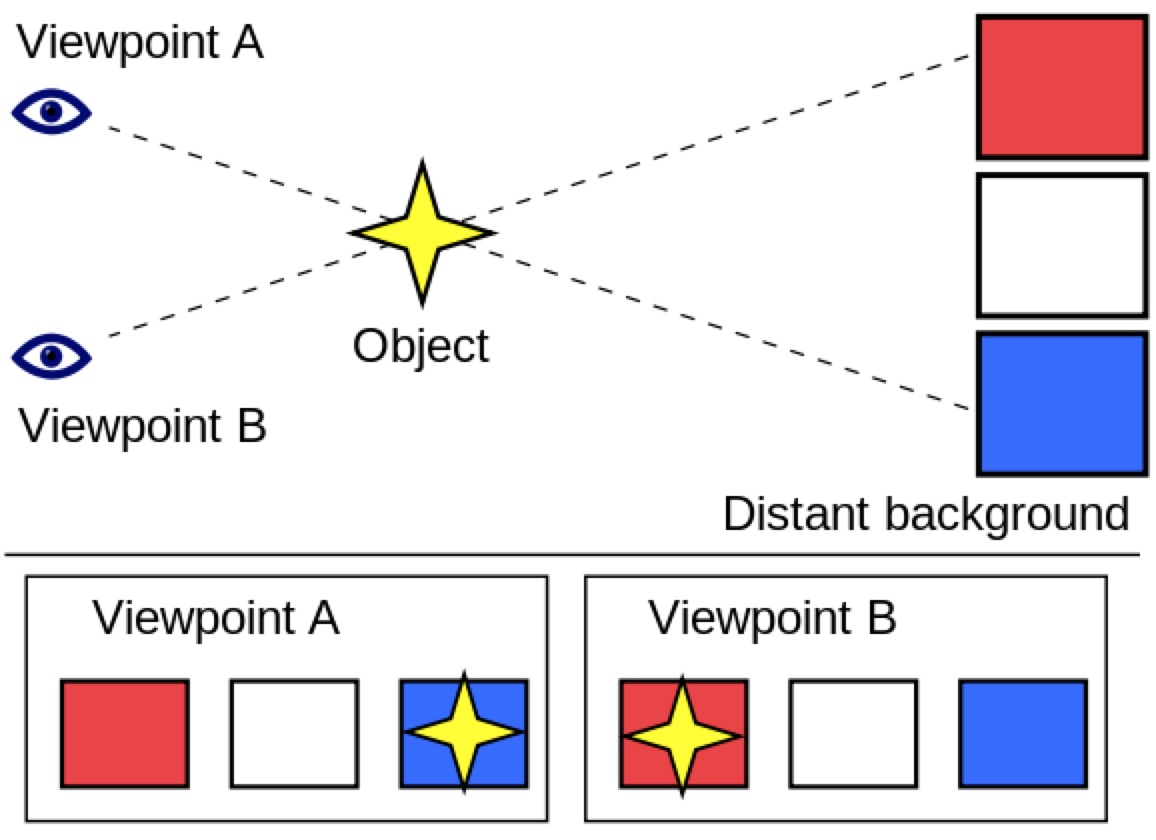
\includegraphics[width=2.5in]{images/ver-acc.jpg}
  \caption{An example of parallax effect.}
  \label{v-aconflict}
  \end{figure}

In non-VR video displays, the screen is bioptic, where only a single display is presented that is viewed by both eyes, so all contents have the same DoF (in this situation the DoF is exactly the distance from eyes to screen) However, in most VR video displays, the screen is stereoscopic, where the illusion of depth is created by delivering images rendered from different angles to each eye. So left eye and right eye receives different image. As a result, in VR display, contents have different DoF.

Fig. \ref{JNDfdof-odof} shows $JND(l, D_o, D_f)$, the JND value for constant luminance = 127, with object's DoF $D_o$ and user's focus distance $D_f$. According to this result, we can verify 2 conclusion above: JND is greater when object has small DoF or object has DoF different from DoF user is focusing on.

\begin{figure}
  \centering
  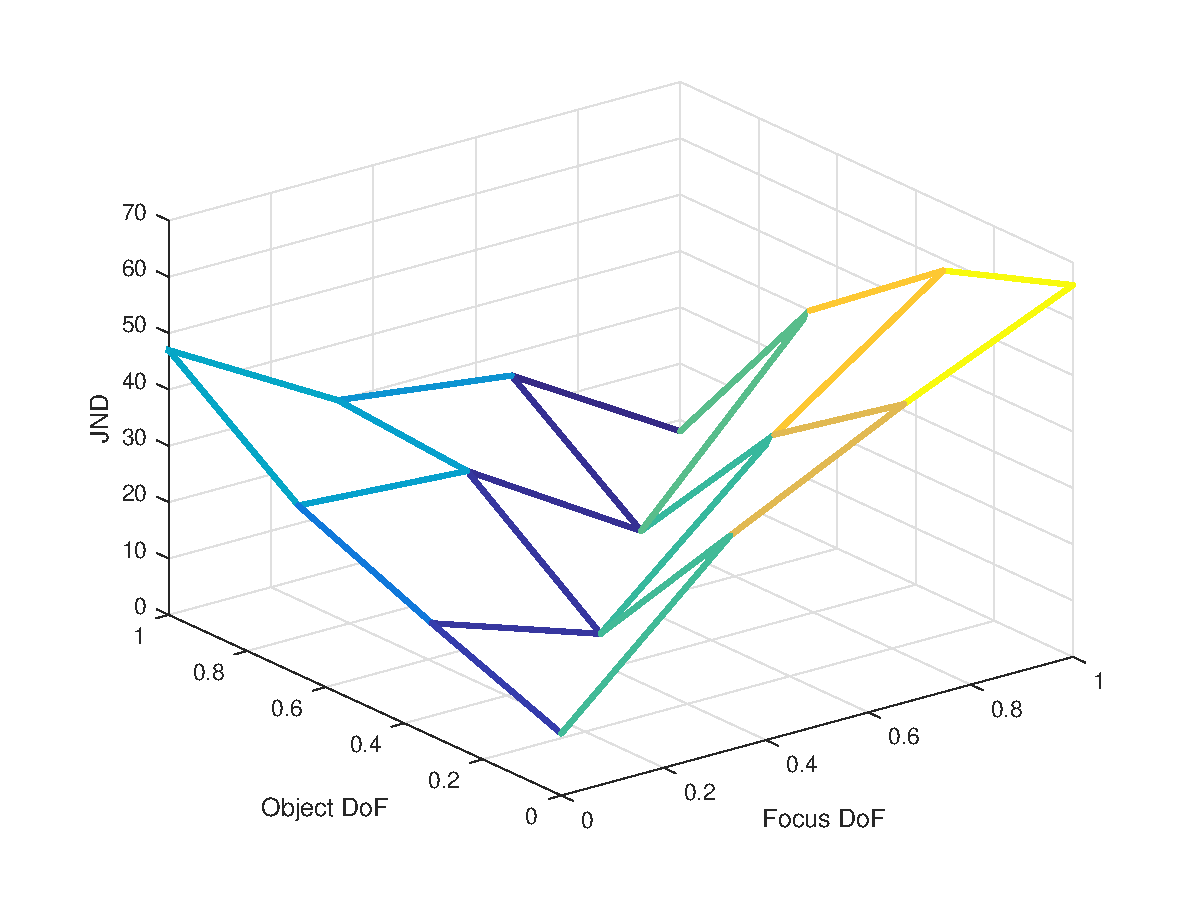
\includegraphics[width=2.5in]{images/JNDfDoF-oDoF.eps}
  \caption{JND due to focus Depth-of-Field and object Depth-of-Field.}
  \label{JNDfdof-odof}
  \end{figure}

To prove the influence of DoF can be considered independently as a coefficient, Fig. \ref{JNDdof-lum} shows $JND(l, D_o)$, the combined effect of object DoF $D_o$ and content luminance $l$ to JND, with $D_f = D_o$. We notice that influence of $D_o$ to JND is very similar in different content luminance. Similarly, we also check whether $D_f$ can be considered independent from luminance $l$ in the same method, and the answer is yes. So the mapping from $l$, $D_o$ and $D_f$ to JND can be decoupled into 2 parts:

\begin{figure}
  \centering
  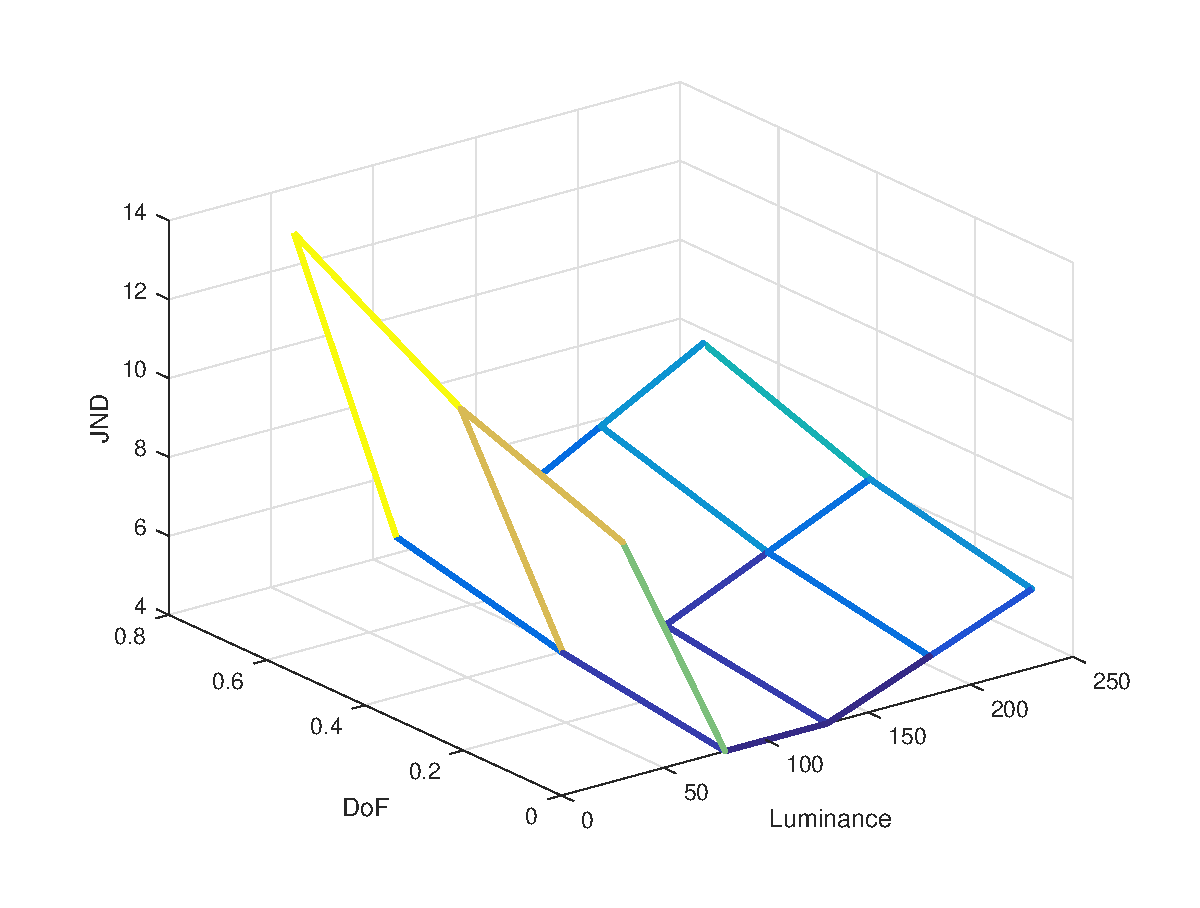
\includegraphics[width=2.5in]{images/JNDdof-lum.eps}
  \caption{JND due to content luminance and object Depth-of-Field.}
  \label{JNDdof-lum}
  \end{figure}

\begin{alignat}{2}\
JND_{lum\&DoF}(l, D_o, D_f) = f_{lum}(l) \times f_{DoF}(D_o, D_f)
\end{alignat}

where $f(_{lum}(l))$ represents the visibility threshold with only consideration of content luminance, and $f_{DoF}(D_o, D_f)$ is a coefficient which represents DoF's influence on visibility threshold.

$f_{lum}(l)$ has been presented as Fig. \ref{JNDluminance}. According to curve fitting, we can obtain $f_{DoF}(D_o, D_f) = \frac{JND_{lum\&DoF}(l, D_o, D_f)}{f_{lum}(l)}$ as Fig. \ref{JNDdof}.

\begin{figure}
  \centering
  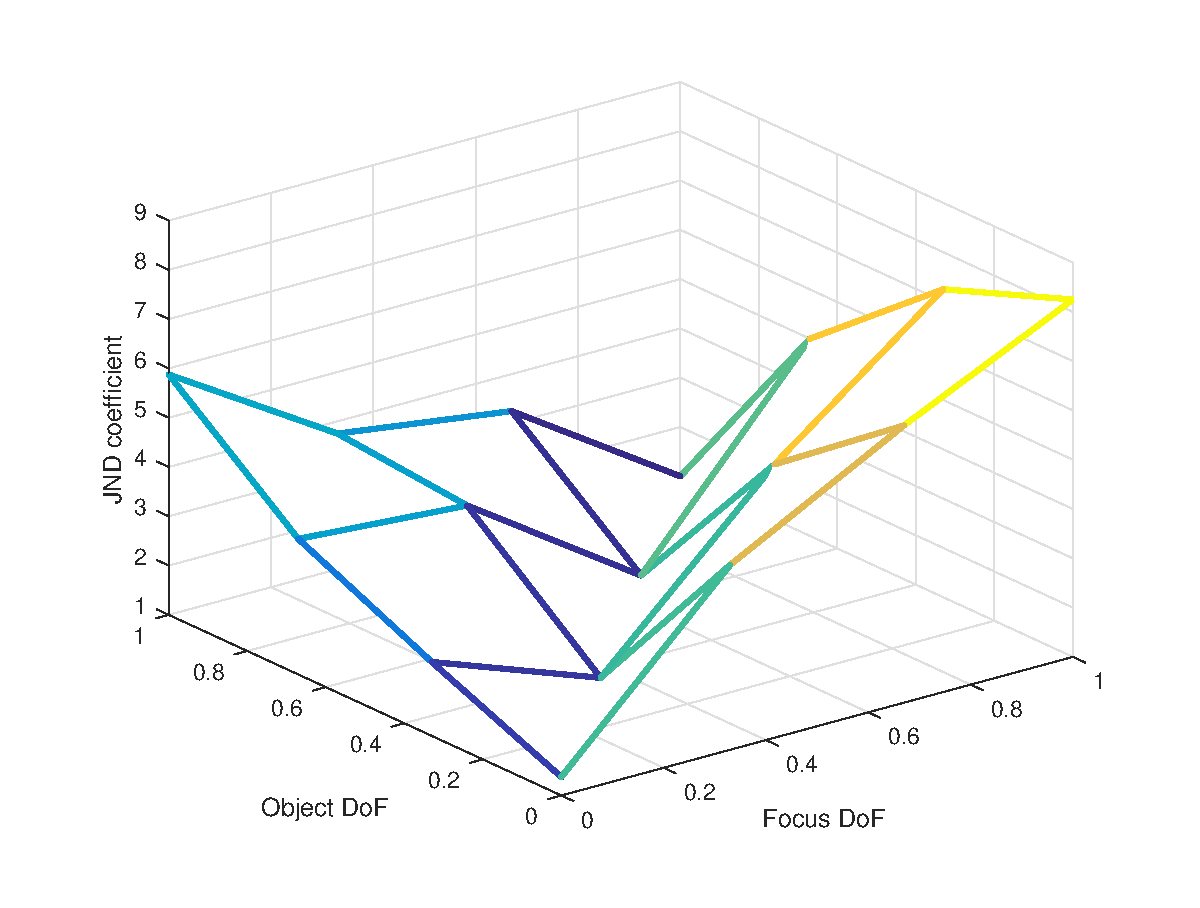
\includegraphics[width=2.5in]{images/JNDdof.eps}
  \caption{$f_{DoF}(D_o, D_f)$, the JND coefficient of object / focus Depth-of-Field.}
  \label{JNDdof}
  \end{figure}

Be similar to viewpoint moving speed in the last subsection, since there is unenviable error in viewpoint prediction, DoF of user focus $D_f$ may be also inaccurate (while $D_o$ is always accurate because it is only video content's property). Fortunately, we analyze the spatial locality of DoF in 50 videos, Fig. \ref{depth_analysis} shows that when the viewpoint predicting error is less than 30 deg, the average error of DoF is below 0.01, and in 87.5\% cases, the error is below 0.013. This viewpoint predicting accuracy can be obtained by current linear regression method.

\begin{figure}
  \centering
  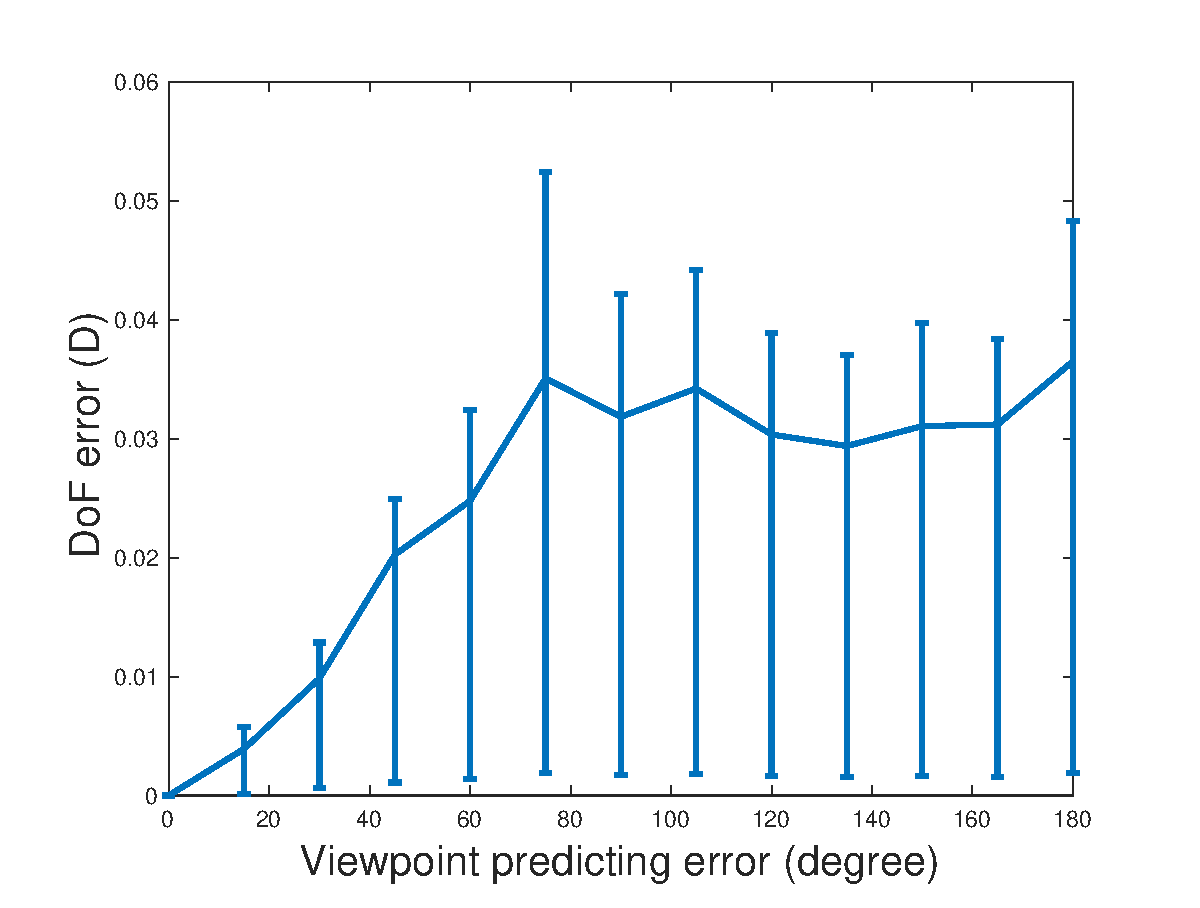
\includegraphics[width=2.5in]{images/depth_analysis.eps}
  \caption{Viewpoint prediction error v.s. DoF error of $D_f$. We present the average error, along with the upper bound and the lower bound of 75\% cases (around the average case).}
  \label{depth_analysis}
  \end{figure}

\subsubsection{JND v.s. luminance \& light / dark adaptation}

In human vision system, in order to transit from day to night vision they must undergo a dark adaptation period in which each eye adjusts from a high luminescence setting to a low luminescence setting. (\cite{darkadaptation}, \cite{darkadaptation2}) Similarly, when human eyes transit from night to day vision they also undergo a light adaptation period. It is well-known that during the process of light / dark adaptation, human visual acuity decreases.

In non-VR video displays, the environment illumination totally depends on the real environment (e.g. under the sunlight, or in a classroom with electric lamp, or in a dark room). However, VR video displays are very different. When user wears HMD, the environment illumination totally depends on video content itself. So when the illumination of video content changes dramatically, eyes need a period of time to adapt the new illumination.

Fig. \ref{JNDadapt-lum} shows $JND_{lum\&ada}(l, \Delta e)$, the combined effect of light / dark adaptation and content luminance to JND. $l$ represents content luminance, $\Delta e$ represents the variation of environment luminance before the test and during the test. 

Be similar to above 2 results, this combined effect can also be decoupled into 2 parts:

\begin{figure}
  \centering
  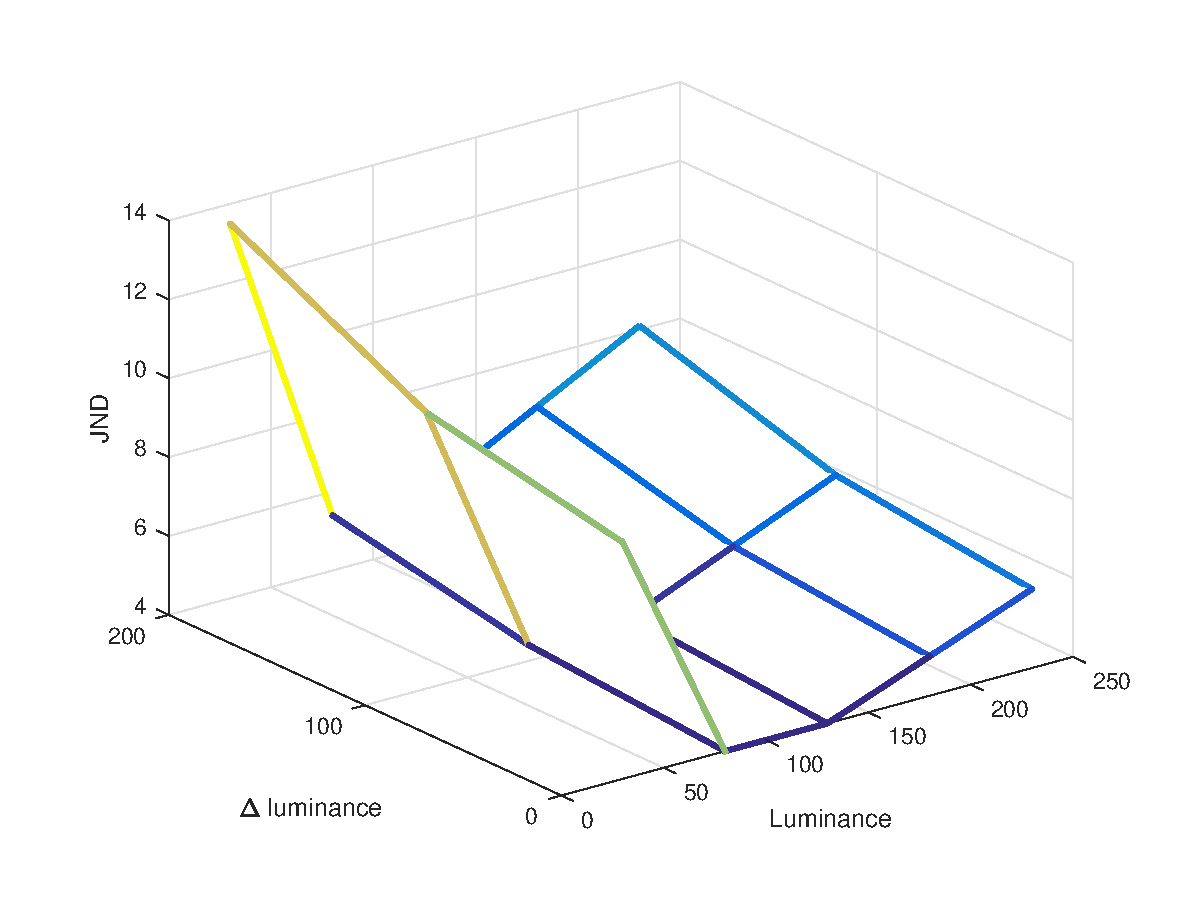
\includegraphics[width=2.5in]{images/JNDadapt-lum.eps}
  \caption{JND due to content luminance and light / dark adaptation.}
  \label{JNDadapt-lum}
  \end{figure}

\begin{alignat}{2}\
JND_{lum\&ada}(l, \Delta e) = f_{lum}(l) \times f_{adapt}(\Delta e)
\end{alignat}

where $f(_{lum}(l))$ represents the visibility threshold with only consideration of content luminance, and $f_{adapt}(\Delta e)$ is a coefficient which represents DoF's influence on visibility threshold.

And we obtain $f_{adapt}(\Delta e) = \frac{JND_{lum\&ada}(l, \Delta e)}{f_{lum}(l)}$ as Fig. \ref{JNDadapt}.

\begin{figure}
  \centering
  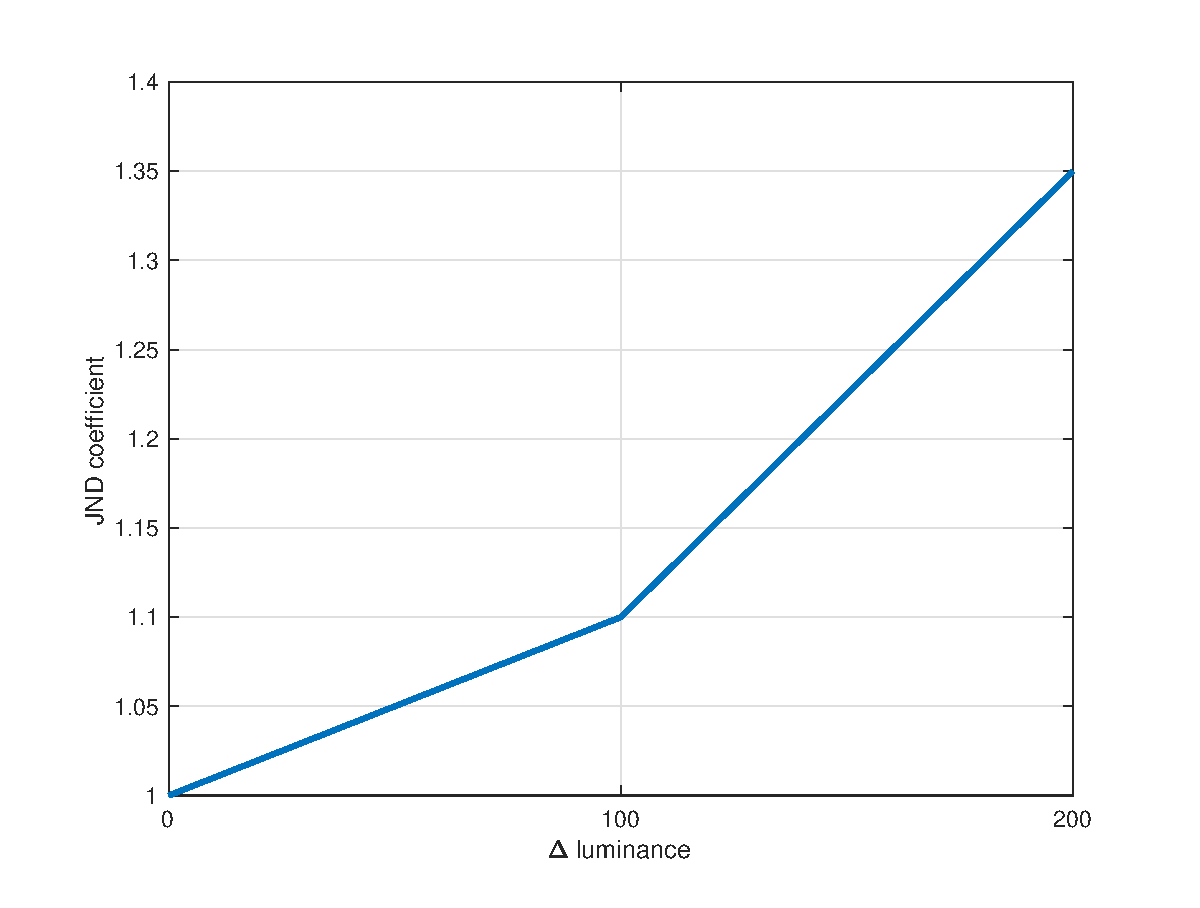
\includegraphics[width=2.5in]{images/JNDadapt.eps}
  \caption{$f_{adapt}(\Delta e)$, the JND coefficient of light / dark adaptation.}
  \label{JNDadapt}
  \end{figure}

\subsubsection{Put it together}

To get the final JND value, we need to put traditional JND factors together with above three new VR-only JND factors. 

Table \ref{table2} lists the symbol and definition used for JND computation.

\begin{table}[h]
\centering
\caption{symbol and definition used for JND computation}\label{table2}
\begin{tabular}{|p{1.5cm}|p{4cm}|p{1.5cm}|}
\hline
symbol & Definition & Source\\
$f_{lum}(l)$ & Visibility threshold due to content luminance $l$. & \cite{PSPNR}, \cite{luminance1}\\
$f_{text}(t)$ & Visibility threshold due to texture complexity $t$. & \cite{PSPNR}\\
$f_{dist}(d)$ & The coefficient of viewpoint-object distance $t$. & \cite{distance}\\
$f_{track}(v), f_{notrack}(v)$ & The coefficient of viewpoint moving speed $v$. & This paper\\
$f_{DoF}(D)$ & The coefficient of Depth-of-Field $D$. & This paper\\
$f_{adapt}(\Delta e)$ & The coefficient of light / dark adaptation $\Delta e$. & This paper\\
\hline
\end{tabular}
\end{table}

For the first 3 JND factors which have been well-studied in traditional video display, measurement of $f_{lum}(l)$ can be found in \cite{luminance1}, measurement of $f_{text}(t)$ can be found in \cite{PSPNR} and measurement of $f_{text}(t)$ can be found in \cite{distance}. We leave the detail of their computation out of this paper.

It is widely accepted \cite{PSPNR} that in non-VR video display, $JND_{nonVR}$ can be computed as follow:

\begin{alignat}{2}\
JND_{nonVR} = \max \{ f_{lum}(l) , f_{text}(t)\} \times f_{dist}(d)
\end{alignat}

Since we have proved that in VR display, 3 new VR-only JND factors, viewpoint moving speed, DoF, light / dark adaptation can be regarded as coefficient on non-VR JND value, $JND_{VR}$ can be computed as:

\begin{alignat}{2}\
JND_{VR} = \max \{ f_{lum}(l) , f_{text}(t)\} \times f_{dist}(d) \times f_{track/notrack}(v) \times f_{DoF}(D) \times f_{adapt}(\Delta e)
\end{alignat}
